\addchapheadtotoc
\chapter{Introduction}
% answer:
% 1) What is the larger context (body of knowledge) for your topic?
% 2) What is the significance of your particular topic?
\section{Named Entity Recognition (NER)}
\subsection{Task Definition}
\label{sec:task}
Named entity recognition (NER) is a fundamental information extraction task that attempts to extract entities from a given text and classify them using pre-defined categories (e.g. persons, locations, or organizations) \citep{2007Survey}. 

Modern approaches to NER use machine learning, using a set of human-annotated, labeled sentences to train a model to classify new sentences. The main dataset I use in this thesis is CoNLL-2003 ~\citep{conll}. This dataset uses a Beginning-Inside-Outside (BIO) format, meaning that each word is classified as either \texttt{B-TYPE} -- the beginning of a named entity, \texttt{I-TYPE} -- any word in a named entity that is not the first, or \texttt{O} -- a non-entity. Separating \texttt{B-TYPE} and \texttt{I-TYPE} helps to distinguish entity boundaries. An example of a labeled sentence appears in Fig~\ref{fig:labeledsent}.

\begin{figure}[h]
	\centering
	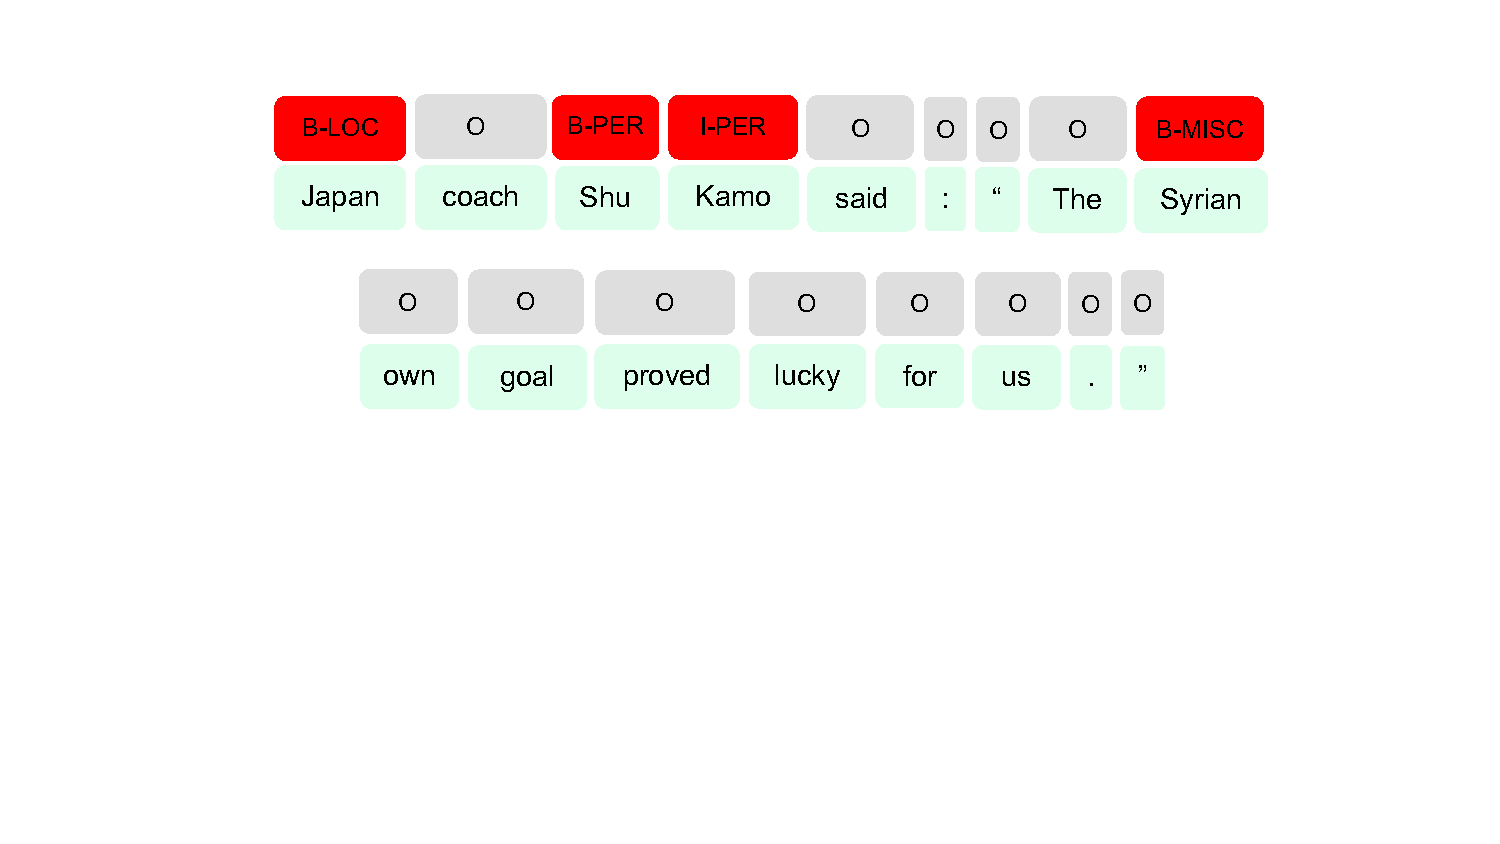
\includegraphics[width=0.85\linewidth]{LatexDiss/figures/labeledsent.pdf} 
	\caption{Example of a human-annotated sentence demonstrating the BIO format.}
	\label{fig:labeledsent}
\end{figure}


More formally, let $\mathbf{x}=[x^{(1)}, x^{(2)}, \cdots, x^{(n)}]$ denote a sentence in the labeled training corpus $\mathcal{D}_{L}$.
Each labeled sentence has a NER-tag sequence $\textbf{y}=[y^{(1)}, y^{(2)}, \cdots, y^{(n)}]$, where $y^{(i)}\in \mathcal{Y}$ and  $\mathcal{Y}$ can be \{\texttt{O}, \texttt{B-PER}, \texttt{I-PER}, \texttt{B-LOC}, \texttt{I-LOC}, $\cdots$\}.
Thus, we have $\mathcal{D}_{L}=\{(\mathbf{x_i}, \mathbf{y_i})\}$, and an unlabeled corpus $\mathcal{D}_{U}=\{\mathbf{x_i}\}$ that we want to label.

In the standard setup, human-annotators are asked to annotate a collection of sentences, which are split into a training, dev, and test set. The CoNLL-2003 dataset is made up of 14,987 training sentences, 3,466 dev sentences, and 3,684 test sentences ~\citep{conll}. The modern approach to NER is using neural models. Sec~\ref{sec:neuralNER} briefly explains the training process of a neural network. During training, the neural NER model has access to each sentence in the training set and its corresponding word labels. The dev set is also used during training. However, the model doesn't directly train on the dev set, but rather uses the dev set to test the model's performance between each training stage. The model predicts labels for the sentences in the dev set, comparing its predictions to the human-annotated labels and adjusting its parameters accordingly. Finally, after the model is completely trained it makes predictions on the sentences in the test set. These predictions are compared to the human-annotated labels, producing an official evaluation of the trained model. The model's performance on the test set is expected to reflect the performance it would have on completely unlabeled sentences.

NER models are evaluated using three different metrics: precision, recall, and an F1 score. Precision measures the rate of false positives by only considering the named entities that the model predicts. Precision is the percentage of the model's predictions that were correct~\citep{conll}. In the case of NER, ``positive'' means that the word is labeled as a named entity.
{
    {
        \begin{align*} 
            \operatorname{P} &= \frac{\operatorname{true\ positives}}{\operatorname{true\ positives} + \operatorname{false\ positives}}
        \end{align*} 
    }
}
Recall only considers the named entities in the dataset. Recall is the percentage of the named entities that the model predicted correctly~\citep{conll}. Precision and recall are depicted in Fig~\ref{fig:evaluationmetrics}.
{
    {
        \begin{align*} 
            \operatorname{R} &= \frac{\operatorname{true\ positives}}{\operatorname{true\ positives} + \operatorname{false\ negatives}}
        \end{align*} 
    }
}
 The F1 score is a combination of precision and recall that is more heavily influenced true negatives, false negatives, and false positives than true negatives \citep{NERevaluationmetrics}. As one can imagine, there should be many true negatives in a NER dataset since the majority of words are non-entities. Because the dataset is more weighted towards negative examples, the F1 score is more effective as an overall measure of the model's performance than a simple accuracy score (the percentage of the model's labels that are correct). The formal definition of the F1 score is as follows:
{
    {
        \begin{align*} 
            \operatorname{F1} &= {(\frac{\operatorname{precision}^{-1} + \operatorname{recall}^{-1}}{2})}^{-1}
        \end{align*} 
    }
}


\begin{figure}[h]
	\centering
	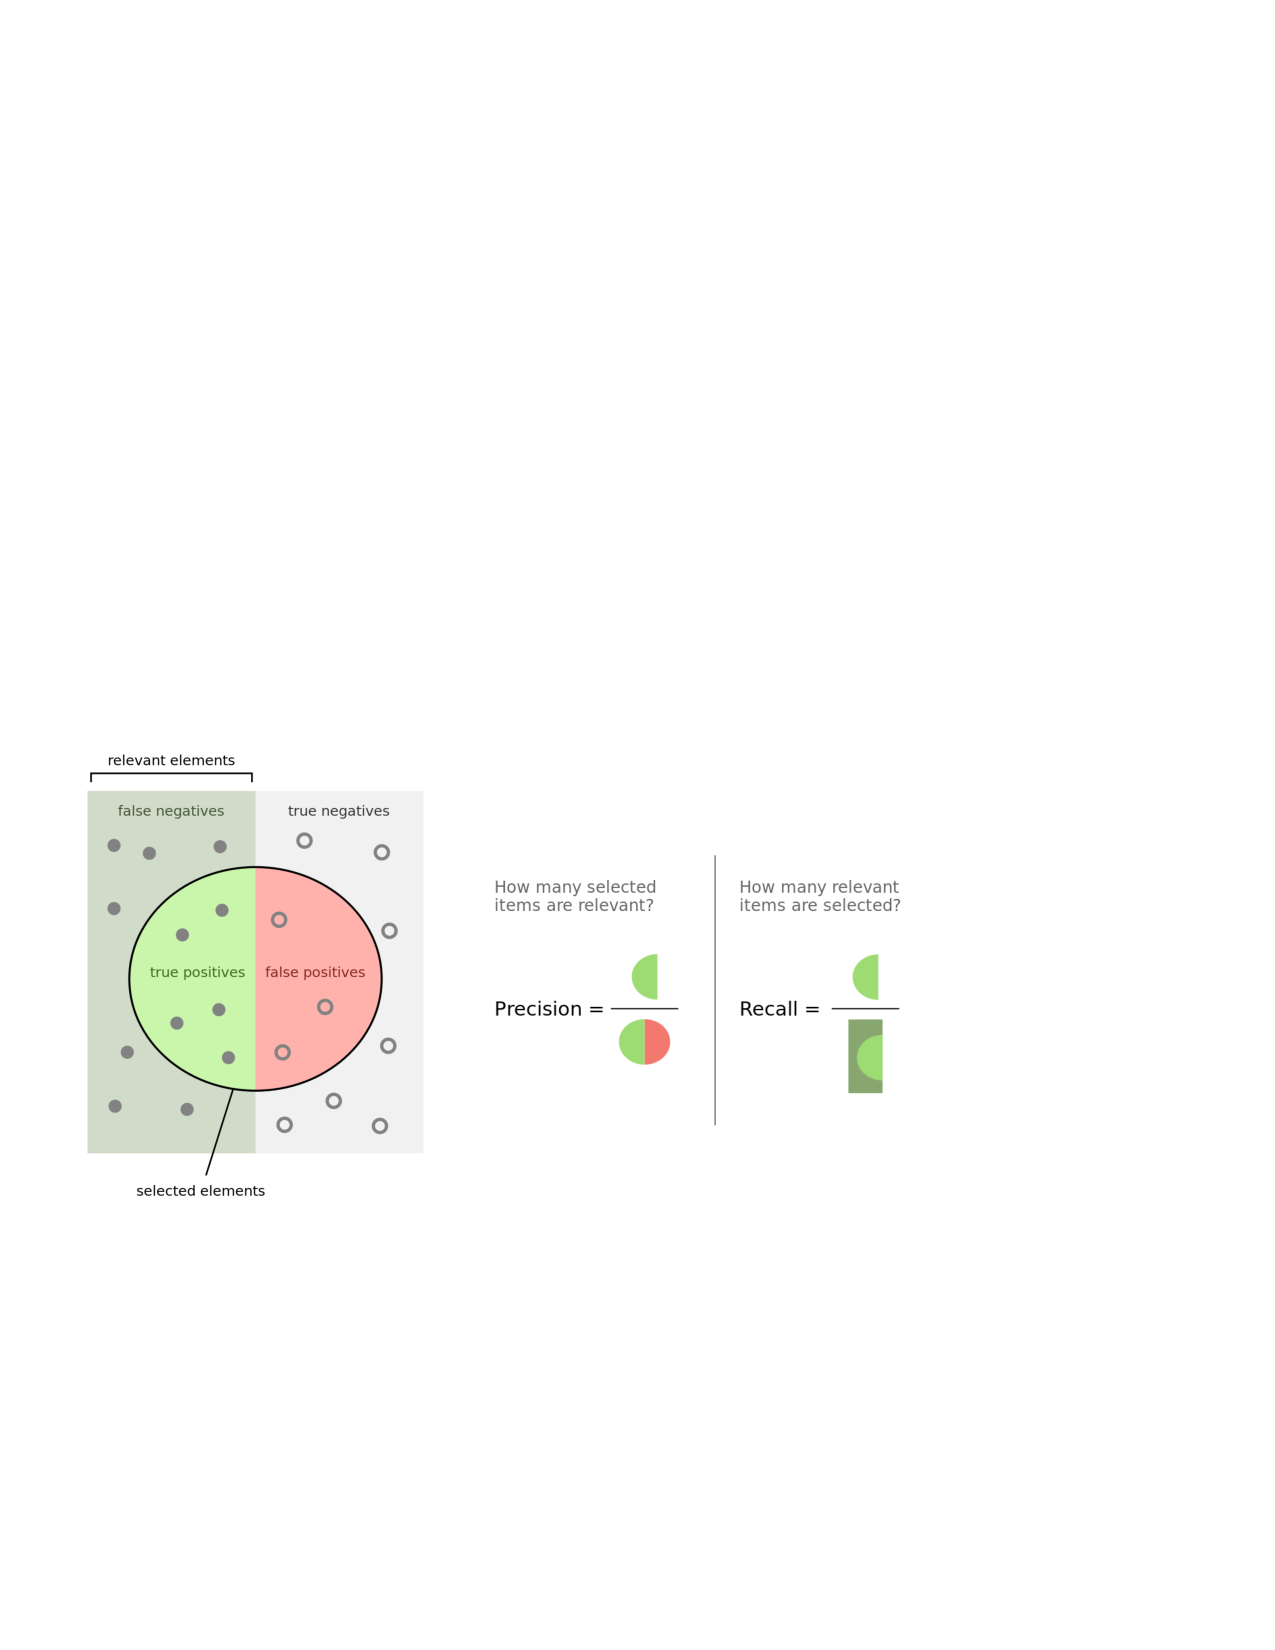
\includegraphics[width=0.85\linewidth]{LatexDiss/figures/evaluationmetrics.pdf}
	\caption{A visual depiction of precision and recall. Figure from~\cite{NERevaluationmetrics}.}
	\label{fig:evaluationmetrics}
\end{figure}

%TODO: do we use strict matching? what about our handling of multiple classes?


\subsection{Neural NER Frameworks}
\label{sec:neuralNER}
Early NER models used hard-coded rules that specified the steps for extracting named entities \citep{NeuralNERSurvey}. Because of their dependence on pre-defined rules, these models were not robust. The next generation of models began to employ machine learning but notably, not deep learning \citep{NeuralNERSurvey}. These models relied on handcrafted feature engineering.
Although an improvement from rule-based approaches, feature engineering still requires researchers to predefine which features are important to their NER model. Examples of such features include which words are capitalized in the sentence, the part of speech of each word, and the frequency of each word within the entire corpus \citep{2007Survey}.

Deep learning using neural networks offers an improvement on these previous approaches by abstracting the definition of rules and features. Neural Networks attempt to model the power of the brain by representing neurons as linear threshold functions that act on a small piece of the input data. By connecting these neurons together, with their weights as trainable parameters, neural networks can represent non-linear functions that act on input data to produce an output prediction. Neural networks learn their non-linear function by repeatedly making predictions on the training data, verifying their predictions, and adjusting the weights of the neurons accordingly. In this way, neural networks learn to make predictions without hand-crafted rules or features; they simply need to be given a large set of training data with the correctly labeled outputs. Since 2011, state-of-the-art NER models have employed neural networks, which outperform previous rule-based and feature-based approaches even without access to external resources and domain-specific knowledge \citep{NeuralNERSurvey}.

\subsubsection{Our Framework}
\label{sec:ourframework}
The basic framework used in this thesis is the most common neural NER architecture, a BLSTM-CRF built on both word and character-level embeddings~\citep{DBLP:conf/acl/MaH16}. The overall structure of this framework is shown in in Fig ~\ref{fig:blstmcrf}. This framework is end-to-end differentiable, meaning that all of the parameters (in the word and character embeddings, the BLSTM, and the CRF) are trained towards the final NER performance.

\begin{figure}[h]
    \centering
    \begin{minipage}[t]{0.5\textwidth}
    	\centering
    	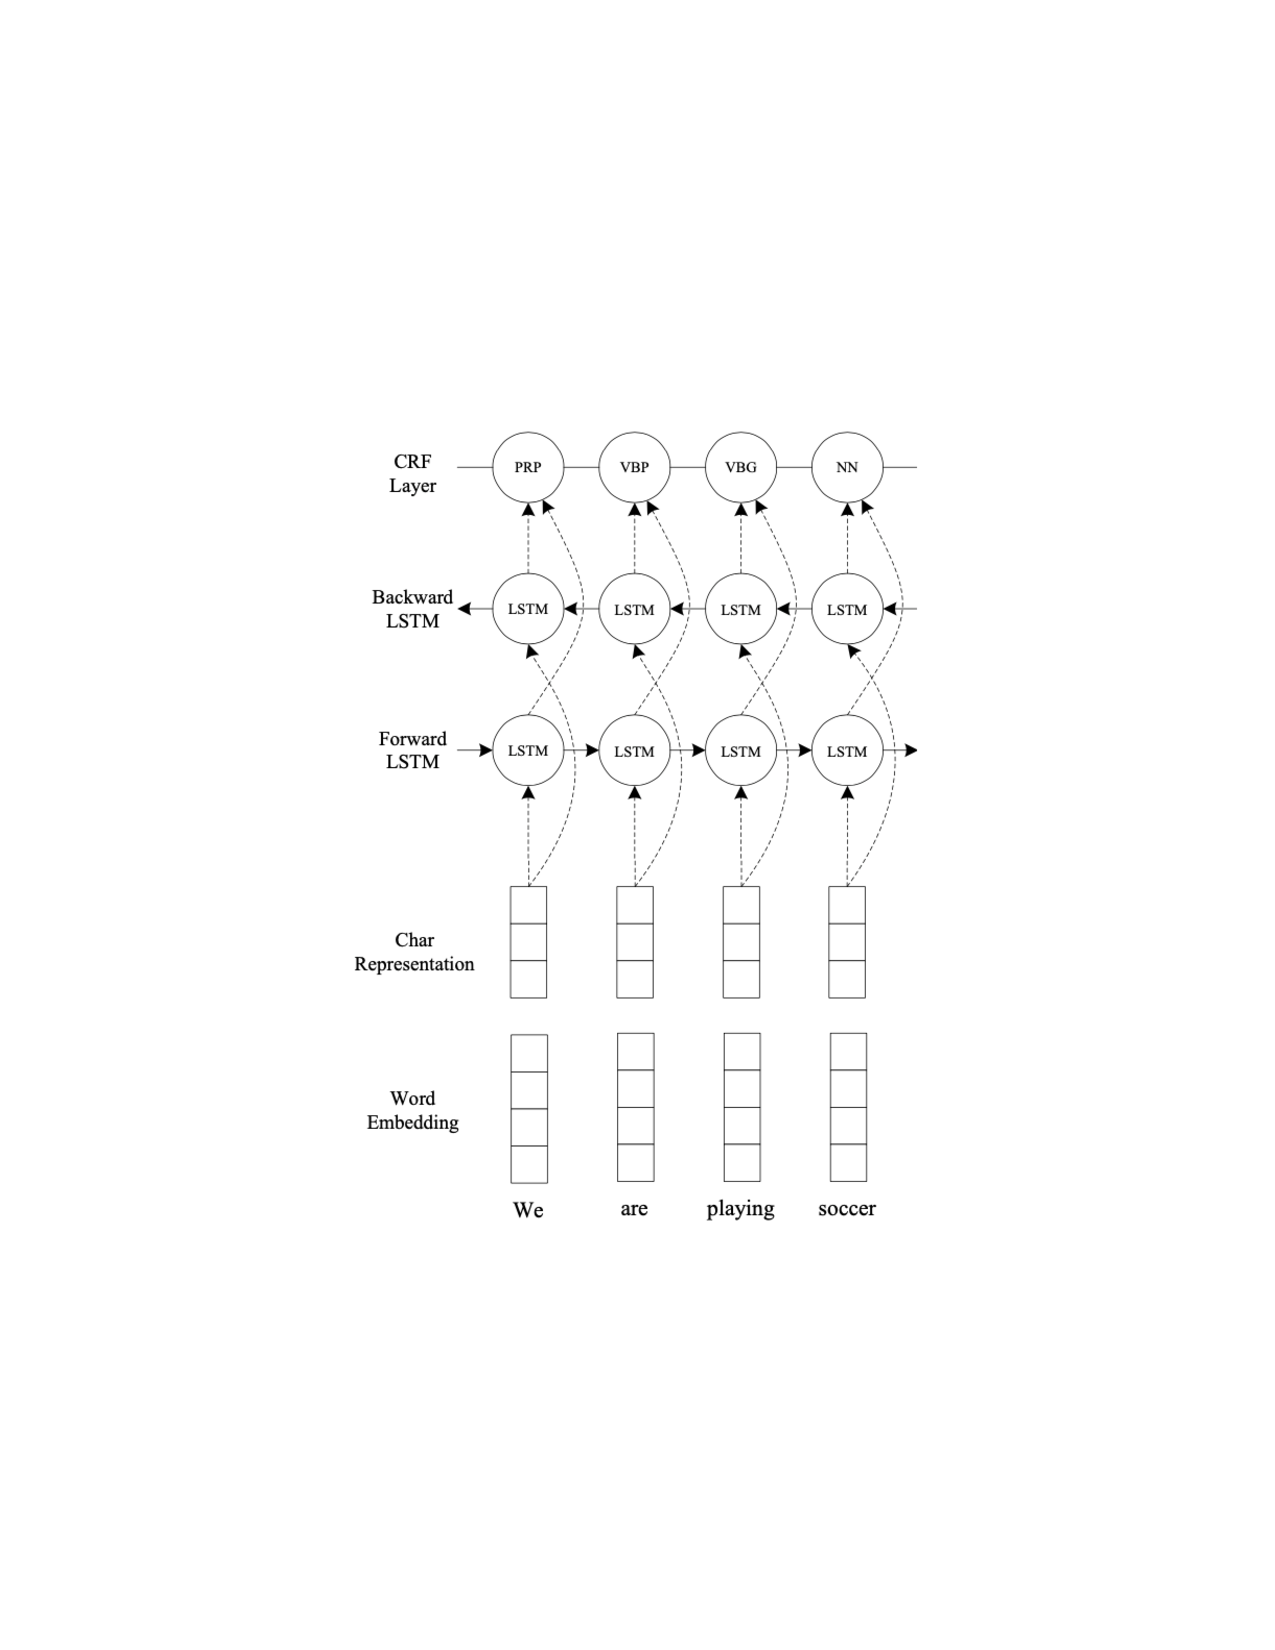
\includegraphics[width=.95\linewidth]{LatexDiss/figures/blstmcrf.pdf}
    	\caption{Overall architecture of neural NER network. Not pictured are the lookup table for word embeddings and the CNN resulting in character embeddings. Figure from ~\citep{DBLP:conf/acl/MaH16}.} %TODO: include self-attention
    	\label{fig:blstmcrf}
    \end{minipage}\hfill
    \begin{minipage}[t]{0.5\textwidth}
    	\centering
    	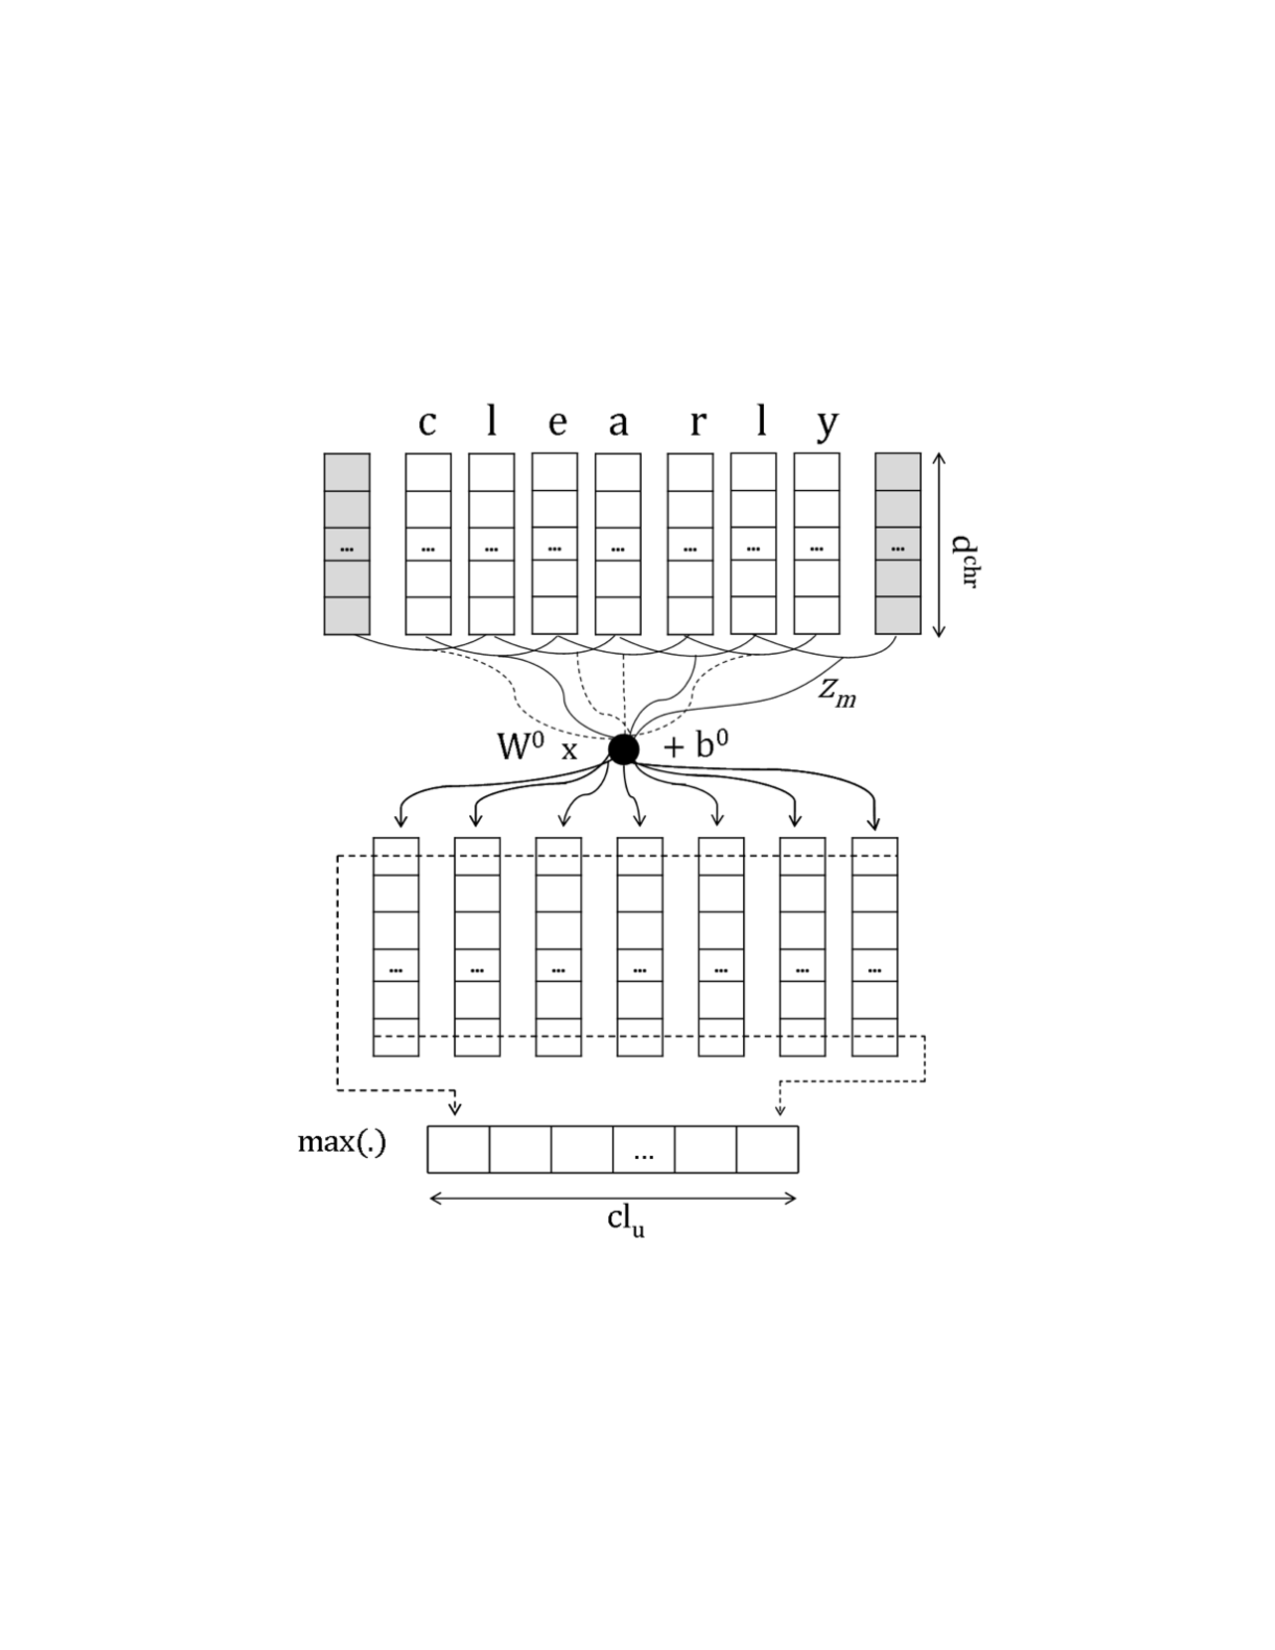
\includegraphics[width=.95\linewidth]{LatexDiss/figures/character-CNN.pdf}
    	\caption{Creating character embeddings using a CNN. Figure from ~\citep{characterembeddings}.}
    	\label{fig:CNN}
    \end{minipage}
\end{figure}

%  TODO ELMO
The first step in our framework is creating word and character embeddings. The purpose of word embeddings is to represent the words semantically; an embedding is a vector representations of a word in a semantic vector space. This means that words that have a small distance from eachother in the vector space should have a similar meaning. We use a lookup table to map each word in our corpus to its embedded vector. In order to speed up the training process, we pre-train the word embeddings using Stanford's publicly available GloVe embeddings ~\citep{Pennington2014GloveGV}. The GloVe embeddings were trained using 6 billion words from Wikipedia and other text on the internet. The meaningful substructure of the resulting  vector space is evidenced by increased performance using GloVe embeddings on a variety of natural language processing (NLP) tasks, including NER and analogy tasks asking ``a is to b as c is to \_?''. By pre-training our word embedding network with GloVe embeddings, the lookup table begins with vectors in the meaningful vector space of the GloVe embeddings rather than starting with a random initialization.

Concurrent with the creation of word embeddings is the creation of character embeddings. Although word embeddings are important for their semantic representation of a word, they leave out useful information regarding word morphology, the actual characters within a word. For example, if a word has the suffix ``ion,'' we can infer that it is probably a noun, while a word ending in ``ing'' is likely a verb. We follow the lead of \cite{characterembeddings}, who use a convolutional neural network (CNN) to create character embeddings, something that had previously been done via handcrafted feature engineering. As depicted in Fig~\ref{fig:CNN}, the characters themselves are passed into the CNN as vectors (representing if the character is a ``c'' or an ``H'' for example). These input vectors are then convolved, meaning that a matrix operation is performed over every window of $k$ neighboring vectors. Convolution is beneficial because characters are morphologically useful in the context of their neighbors. We then extract a single character embedding vector for the word using max pooling over the convolved vectors. 

After creating the character and word embeddings, the two vectors are concatenated and fed into a bi-directional long-short term memory (BLSTM) neural network~\citep{DBLP:conf/acl/MaH16}. When making labeling predictions, a vanilla neural network would only have access to the word in question. Because it would not have access to any of the surrounding words, a vanilla neural network is unable to take advantage of contextual clues in the sentence. LSTMs provide access to previous words in the sentence by using the previous words' LSTM outputs as inputs, proportionally ``forgetting'' the most distant words. In NER, it is useful to have access to both the past words and the future words in a sentence. Because of this, we use a bi-directional LSTM. As depicted in Fig~\ref{fig:blstmcrf}, a BLSTM consists of a forward LSTM (which evaluates the sentence from left to right) and a backward LSTM (which evaluates the sentence from right to left). When evaluating a given word, the forward LSTM has access to the past context while the backwards LSTM has access to the future context. The outputs of the forward and backward LSTMs for a given word are concatenated to form the final output of the BLSTM for that word.

Finally, we are ready to perform label prediction on our word.
If we directly used the BLSTM output to predict our labels, we would have to make each word's prediction individually. We prefer to jointly label the words in a sentence because their labels are highly correlated. For example, it is highly unlikely that a word tagged as an organization entity would be directly followed by a person entity without any non-entity words in between. In order to jointly label the words of a sentence, we use a conditional random field (CRF) as our final network layer ~\citep{DBLP:conf/acl/MaH16}. Rather than choosing the highest probability label for an individual word, the CRF maximizes the log-likelihood of the sentence's entire sequence of labels. This can be done efficiently using the Viterbi algorithm ~\citep{ViterbiAlg}.

Another concept that is important to our framework is attention. Attention allows an external context vector to scale a word's hidden state vector, emphasizing some dimensions while demphasizing others. 
Given an input word's hidden state $\vec{h_t}$ and word-level context vector $v^{T}$ as well as trainable parameters $\mathbf{W}$ and $\vec{b}$, the attention vector $\vec{\alpha_t}$ is computed as follows~\citep{understandingattention}.

{
    {
        \begin{align*} 
            \vec{u_t} &= \tanh (\mathbf{W} \vec{h_t} + \vec{b}) \\
            \vec{\alpha_t}  &= \operatorname{SoftMax}(v^{T} \vec{u_t})
        \end{align*} 
    } % use equations from self-attention paper instead?  I think these are more straightforward.
}

Geometrically, $\mathbf{W}$ and $\vec{b}$ rotate and scale the  word's hidden state vector. Then, the $\tanh$ function stretches components of the vector. The external context vector $v^{T}$ represents the relative importance of each dimension of the new vector $\vec{u_t}$. Taking the dot product of $v^{T}$ and $\vec{u_t}$ scales each component of $\vec{u_t}$ by its dimension's weight in $v^{T}$. Because $W$ and $\vec{b}$ are trainable parameters, the model learns how to manipulate the word's hidden state vector so that its dimensions are most effectively scaled by $v^{T}$. Finally, the $\operatorname{SoftMax}$ function turns the resulting attention vector into a probability distribution, normalizing each element.

Attention is particularly useful when we want to incorporate external information because this information can be included as the context vector (as we do in Sec~\ref{sec:secondstage}). However, attention can also be used in the absence of external information through self-attention. In self-attention, a word's hidden state vector is itself used as the context vector $v^{T} = h_t^{T}$~\citep{selfattentive}. The resulting attention vector focuses on a specific semantic component of a sentence (such as a set of related words). Because a sentence often has multiple important components, self-attention can be computed $k$ times with a different set of parameters for each, resulting in an attention matrix. % TODO: why does self-attention work intuitively?

\section{Problem Statement}
Neural NER models are powerful in settings in which an abundance of ground-truth training data is available \citep{LampleNER}. However, human annotation is expensive and time-consuming, especially in technical domains, such as biomedical publications, in which the human annotator must be able to understand and contextualize technical jargon. Unfortunately, neural NER model performance decreases significantly when training data is restricted \citep{TriggerNER}. Thus, a crucial research question is how we can most efficiently collect and use human-annotated ground-truth data. In this thesis, I investigate two potential solutions. First, I explore a novel way of collecting human-annotated data by gathering both ground-truth entity labels and \textit{entity triggers} -- the phrases which cue entities. This approach allows for state-of-the-art results using a smaller set of human annotations. Second, I explore automated methods to create adversarial data to evaluate models and additional training data without any additional human input.

\subsection{Entity Triggers}
\subsubsection{Our approach}
As a method to more efficiently collect human annotations, I worked with USC's Intelligence and Knowledge Discovery Research Lab to introduce \textit{entity triggers} \citep{TriggerNER}. We hypothesize that collecting human explanations of the annotators' choices in entity labels could provide a more label-efficient learning of NER models. An entity trigger is a group of words in a sentence that helps to explain why a human would recognize an entity in the sentence. For example, in the sentence ``He ate lunch at IHOP,'' \textit{ate lunch at} is an trigger phrase for the entity \textbf{IHOP}. After collecting human annotations for both entities and entity triggers we train a neural network to predict entity triggers in unlabeled sentences. We use these predicted entity triggers as additional supervision for the final goal of predicting entities. Our experiments demonstrate the cost effectiveness of using entity triggers. Training our framework on only 20\% of the trigger-annotated training sentences results in a comparable performance to conventional approaches using 70\% of the training data.

\subsubsection{Related Works}
% ~\citep{weaklabel} created automatically labeled NER data for a target language via annotation projection on comparable corpora. Then, they filter out weakly labeled (WL) sentences by statistical methods. However, this paper regards unlabeled words as 'O' so that it cannot deal with incomplete annotation. 
Towards low-resource learning for NER,
recent works have mainly focused on dictionary-based distant supervision, using a dictionary of entities and an unannotated target domain corpus to generate weakly labeled data, data which we have less confidence in because it was not annotated by hand. This approach uses exact character matchings of words in the unannotated corpus with entities in the entity dictionary, regarding the hard-matched sentences as additional, weakly labeled data for learning a NER model. 
~\cite{autoner} and ~\cite{yangner} follow this approach, employing Partial CRFs to tentatively assign unlabeled words all possible labels, choosing the pattern that maximizes the total probability. One drawback to their approach is that they rely on a domain-specific seed dictionary. 
~\cite{weakcrf} use Wikipedia anchors, assumed to be named entities, as their entity dictionary. Using the Wikipedia anchors, they automatically construct weakly labeled data, splitting them into high-quality and noisy data. Then, they train a classification module, which regards name tagging as a multi-label classification problem. This module uses noisy data first and fine-tunes with high-quality data. After pre-training this classification module, they share the overall neural network with the sequence labeling module. Then, they use a sequence labeling module to infer the named entity. This paper does not rely on a domain-specific seed dictionary, but it relies on Wikipedia. One drawback is that their weak labeling method doesn't consider the context of a sentence.
~\cite{opencorrection} similarly construct weakly labeled data from Wikipedia and DBpedia. Using a small amount of human annotated data, they implement a semi-supervised correction model with curriculum learning to correct the false-negative entity labels in the weakly labeled data. Finally, they use the corrected data to train a neural NER model. They show the effectiveness of curriculum learning using weakly labeled data, but it can only be applied to general NER tasks such as CoNLL. It cannot be applied to domain-specific tasks such as medical text.

Although the dictionary-based approaches largely reduce human efforts in annotating, the quality of matched sentences is highly dependent on the coverage of the dictionary and the quality of the corpus.
The learned models tend to have a bias towards entities with similar surface forms as the ones in the dictionary. Without further tuning under better supervision, these models have low recall.
Unlike these works aiming to get rid of training data or human annotations, our work focuses on how to more cost-effectively utilize human efforts.

Another line of research which also aims to use human efforts more cost-effectively is active learning~\citep{shen2018deep,Lin2019AlpacaTagAA}.
This approach focuses on instance sampling and the human annotation UI, asking workers to annotate the most useful instances first.
However, a recent study~\citep{Lipton2018PracticalOT} argues that actively annotated data barely helps when training new models. 

Inspired by recent advances in learning sentence classification tasks using explanations (i.e. human-written rules)~\citep{Li2018GeneralizeSK, Hancock2018TrainingCW, Wang2020Learning, Zhou2019NEROAN} such as relation extraction, we propose the concept of an ``entity trigger'' for NER.
These prior works primarily focus on sentence classification, in which the rules are continuous token sequences and there is a single label for each input sentence.
The unique challenge in NER is that we have to deal with rules which are discontinuous token sequences and there may be multiple rules applied at the same time for an input instance. Our work using entity triggers sheds light on future research directions for more cost-effectively learn NER models.


\subsection{Generating Adversarial Data}
\label{sec:introadv}
\subsubsection{Adversarial Examples}
An adversarial example for a neural network is an example that is created by perturbing a correctly classified example, causing the model to misclassify the  adversarial example. Adversarial examples are easily understood within the image domain, where a slight rearrangement in the pixels of an image results in a new image that is almost indistinguishable to a human (and thus would be classified the same as the original image). A classic example in pop-science is the slight rotation of an image of a tabby cat. Google's image classifying network is over 80\% confident the original image is a cat. However, with the slight rotation, the network becomes 90\% confident that the same image is a bowl of guacamole \citep{guacamole}. Adversarial examples in the natural language domain are slightly more complicated because rearranging words or characters in a sentence doesn't always result in a sentence that is syntactically valid, let alone semantically similar to the original sentence. I explore several ways to perturb sentences such that the original entity labels and the sentence structure both remain valid.

Adversarial examples are useful in part because they demonstrate the limits of state-of-the-art NER models. By creating adversarial data to effectively trick a NER model, we develop a better idea of the model's brittleness, which can guide future research directions for making the model more robust. Adversarial examples are particularly important because test data is usually collected in a similar manner as the training and dev data, so models are biased towards that particular writing style~\citep{SEARs}. When used in real-world applications, using brittle models can be dangerous.

My experiments demonstrate that the algorithms I develop to generate adversarial examples are effective at fooling state-of-the-art NER models.

\subsubsection{Adversarial Training}
Another use of adversarial examples, the use that I focus on in this thesis, is data augmentation by adversarial training. By developing scripts to create adversarial examples, I've effectively developed scripts to take a set of labeled data and produce additional, slightly different, labeled data. I hypothesize that since the adversarial examples of our test data are able to trick our NER models, the adversarial examples must have implicit knowledge that the NER model currently lacks, knowledge which could improve the NER model if it was embedded into the training data. With this in mind, I use the same scripts for creating adversarial examples to augment the training data, creating more, slightly different, training data without additional human annotation cost. This approach --  augmenting the training data using techniques for generating adversarial test examples -- is called \textit{adversarial training}.
My experiments show that adversarial training improves the NER models' robustness to adversarial attacks while retaining its effectiveness on the original test data sets. 


\subsubsection{Related Works}
Most of the research on adversarial examples for neural networks has been performed within the image domain. Within NLP, there has been little research on adversarial examples within NER specifically. However, recent research on adversarial examples within other subcategories of NLP inspires this thesis.

\cite{alzantotAdver} use genetic algorithms to create adversarial examples via word substitutions for sentiment analysis and textual entailment tasks. Their attacks cause standard  models to make errors with a rate of 97\% and 70\% respectively. Further, over 90\% of their adversarial examples were correctly classified by humans, evidencing the validity of their attacks. They found that adversarial training did not result in models robust to their adversarial attacks.

\cite{jiaadver} create adversarial examples for the Stanford Question Answering Dataset by inserting random sentences into the paragraphs that the model is asked a question about. They find that the model's accuracy drops from an F1 score of 75\% to 36\%. They find that adversarial training increases the model's accuracy on the adversarial test set to 70\%. However, the adversarial training does not offer robustness beyond  their specific attack; when they train the model with extraneous sentences added to the end of the paragraph, it performs poorly on data with a sentence added to the beginning, reaching only a 39\% F1 score.

By using back translation to create paraphrased training data, \cite{paraphraseadver} develop an encoder-decoder model to produce a paraphrase of an input sentence conforming to a specific inputted syntactic pattern. This paraphrasing model is then used to produce adversarial examples for sentiment analysis. Because their paraphrasing model makes dramatic structural changes to the input sentence rather than minor lexical substitutions, \cite{paraphraseadver} find that their model creates more convincing adversarial examples than uncontrolled paraphrasing models. Their paraphrasing model creates adversarial examples which cause the sentiment analysis model to fail on 33\%/41\% (depending on the specific task) of paraphrases of originally successful test examples. In comparison, the adversarial data  generated by uncontrolled paraphrasing models only breaks 20\%/20\% of the sentiment analysis test examples. Adversarial training reduces the percentage of broken test examples from 33\%/41\% to 20\%/31\%.

% Iyyer et al., 2018 another example
% Belinkov and Bisk, 2017 another example (noise and typos)

Another example is the research done by \cite{certifiedrobustness} on adversarial word substitutions for sentiment analysis tasks. They focus on training a model to be robust to word substitution attacks on test data. They note that their main challenge is knowing what the best (i.e. hardest) adversarial attacks are despite an exponentially sized set of possible perturbations. They use an algorithm called Interval Bound Propagation (IBP) to tractably compute an upper bound for the model's error considering the worst-case adversarial attack, and they set the training goal to be minimizing the upper bound on the worst-case error. They find that this mathematical approach is even more effective than adversarial training via direct data augmentation. Direct data augmentation alone raised the models' accuracy on adversarial test data from 6.9-9.6\% using models trained on standard data to 33.0-35.2\% using models trained on augmented data. Although this is a major achievement, supporting the effectiveness of data augmentation, their mathematical approach using IBP raises the models' accuracy to 64.7-75.0\% \citep{certifiedrobustness}.

The research of \cite{SEARs} comes closest to my work on adversarial examples and adversarial training, although they work in the fields of machine comprehension, visual question-answering, and sentiment analysis rather than NER. Because of the fields they work in, their adversarial perturbations must retain both sentence validity and semantic similarity. Thus, their adversarial examples are \textit{SEAs} (semantically equivalent adversaries) which they generalize into the rules that produce them, \textit{SEARS} (semantically equivalent adversarial rules). Examples of SEARs include changing \textit{``What is...''} to \textit{``What's...''} or chaging \textit{``What \textsc{NOUN}...''} to \textit{``Which \textsc{NOUN}...''}. The SEARs are shown to create far more numerous and more effective SEAs than humans writing SEAs directly. They then use the SEARs for adversarial training. This  resulted in an insignificant change in performance on the original test data and a significantly lower error rate on the SEAs, from 12.6\% to 1.4\% for visual question answering and 12.6\% to 3.4\% on sentiment analysis~\citep{SEARs}. This project in particular motivates my research in adversarial training.

Adversarial examples for NER is a relatively untouched field. However, there are a few recent pieces in that direction. \cite{entityswitched} released a manuscript in April 2020 regarding entity-switched datasets for NER. It has not yet been peer-reviewed. The idea is that NER models should be able to recognize named entities from a variety of national origins equally well. This follows recent research on fairness in machine learning\footnote{For example, language identification models are poor at recognizing African-American Vernacular English as English despite their high performance recognizing text as English when associated with white speakers~\citep{blodgett2016}}. To investigate NER model robustness across national origins, they switch out entities in the CoNLL03 dataset, replacing them with entities of a different national origin. They find that state-of-the-art models have significantly unequal performance across national origins, ranging from a recall of 99.6-99.7\% on US-based named entities to only 78.2-84.2\% on Vietnamese-based named entities. 

\cite{interpretability} is another example of recent research in adversarial data for NER. This manuscript was released in April 2020 and has not yet been peer-reviewed. They attempt to address the question of whether state-of-the-art NER models are learning the context of named entities or are merely memorizing the named entities in the training data. In order to investigate this question, they test the ability of state-of-the-art models to label words given only the context of the word. The models are asked to label sentences of the form ``\textit{Tom traveled to \_\_\_ last year.}'' A  sentence is created for each word in the CoNLL03 dataset, with that word blanked out. This context-only approach is similar to the data augmentation technique of entity masking that I explore, where I replace each entity with a random string of letters. \cite{interpretability} find that models have an F1 score of above 90\% given words and context, 50-60\% given context only, and 65-80\% given the single word only. This suggests that modern models rely more heavily on memorizing named entities than learning the context for named entities. Interestingly, human tests demonstrate that many of the mistakes that the models make during context-only labeling are also made by humans given the context-only sentence. For example, in the sentence \textit{``Their other marksmen were Brazilian defender Vampeta \_\_\_ Belgian striker Luc Nilis''} the actual blanked word is \textit{``and''}, so it should be labeled with the tag \textsc{O}. However, the models and human annotators alike labeled the word \textsc{PER}. This is relevant to my research because it suggests the possibility that some of my augmented sentences could be too difficult for human annotators. If this were the case, it would be unreasonable to expect models to correctly label these sentences.

Finally, \cite{biomedadv} is yet another manuscript on adversarial data for NER released in April 2020. It also has not yet been peer-reviewed. They focus on the biomedical corpora. They have two main attack strategies. First, they mimic typos by either swapping neighboring characters in a word or replacing a character with a character that is nearby on a keyboard. This is different from my approach in that it yields sentences that are grammatically incorrect. However, because they are small perturbations, humans could still annotate the adversarial sentences correctly. Their second approach is to replace chemical and disease names with synonyms. This is different from my approach because they are replacing the actual named entities themselves (chemical and disease names) with synonyms whereas I replace non-entities with synonyms. They find a significant drop in state-of-the-art NER models' performance on these adversarial examples, with the F1 score dropping 20\%-50\%. Adversarial training helps the models' performance on the adversarial examples. However, it also negatively impacts the models' performance on the original test data.


%from Truecaser:
% Although modern named entity recognition (NER) systems show impressive performance on standard datasets, they per- form poorly when presented with noisy data. In particular, capitalization is a strong signal for entities in many lan- guages, and even state of the art models overfit to this feature, with drastically lower performance on uncapitalized text. In this work, we address the problem of robustness of NER sys- tems in data with noisy or uncertain casing, using a pretrain- ing objective that predicts casing in text, or a truecaser, lever- aging unlabeled data. The pretrained truecaser is combined with a standard BiLSTM-CRF model for NER by appending output distributions to character embeddings. In experiments over several datasets of varying domain and casing quality, we show that our new model improves performance in un- cased text, even adding value to uncased BERT embeddings. Our method achieves a new state of the art on the WNUT17 shared task dataset.